\chapter{Discussion}
\label{Chap5}
\section{Powder ageing}
\subsection{Grain size and distribution}

Two trends were identified in section \ref{RGSAD}: there was a clear diminution of the average particle size $D_a$ and a narrowing of the distribution as functions of the number or recycling cycles. Only one sampling did not concur with these observations. This can be easily explained: the powder in question was sampled just after fresh powder was added to the recycled one. The distribution was thus altered in a way that is opposed to what recycling causes.\\

[D'ou viennent les tendances?]\\

Furthermore, ultrasonic treatments gave the opportunity to discover that a non-negligible part of the AlSi10Mg powder agglomerated, with particle sizes going up to 134 [$\mu m$]. It seems reasonable to assume that the agglomerates could have lead to the emergence of defects in the fabricated parts. This could, at least partly, explain the scatter of relative densities for samples from a same batch. It may also be a reason behind the remarkably poor properties of sample "8a" (see section \ref{RReprod}).\\
\subsection{Composition}
[Mg connu pour s'évacuer]

\section{Density measures assessments}
\label{DDMA}

%\subsection{Hydrostatic weighing}


\subsection{Relative optical density image analysis}
\label{DRODIA}

The estimation of the relative density through RODIA can be distorted on many grounds. First, the distribution of porosities is inhomogeneous on the analysed surface. Multiple photos must thus be taken with a systematic manner for each specimen to constitute a representative sample.\\

Second, the quality of the photographs has a critical role. The isolation of the porosities during the thresholding requires a substantial difference of pixel intensity between the holes and the material. Since some porosities and some zones of the material can appear respectively brighter or darker than was is expected, there are risks that one isolates spots and/or not actual porosities. Additionally, the thresholding is manual and thus prone to slight human errors. \\

Most importantly, the finite resolution of the camera implies that sufficiently small porosities are not visible on the pictures. 

One can expect the the density measurement through RODIA to be a biased method, due to the discretisation in pixels among other things. Results for pictures with different magnifications were compared to quantify these effects. For this purpose, a picture was taken under 5x magnification and two under 10x magnification. The former was delimited to match the visible zones on the latter (see figure \ref{fig:RODIA1}). The same two zones - named A and B - were thus analysed for different levels of resolution.\\

\begin{figure}[ht]
	\centering
	\centerline{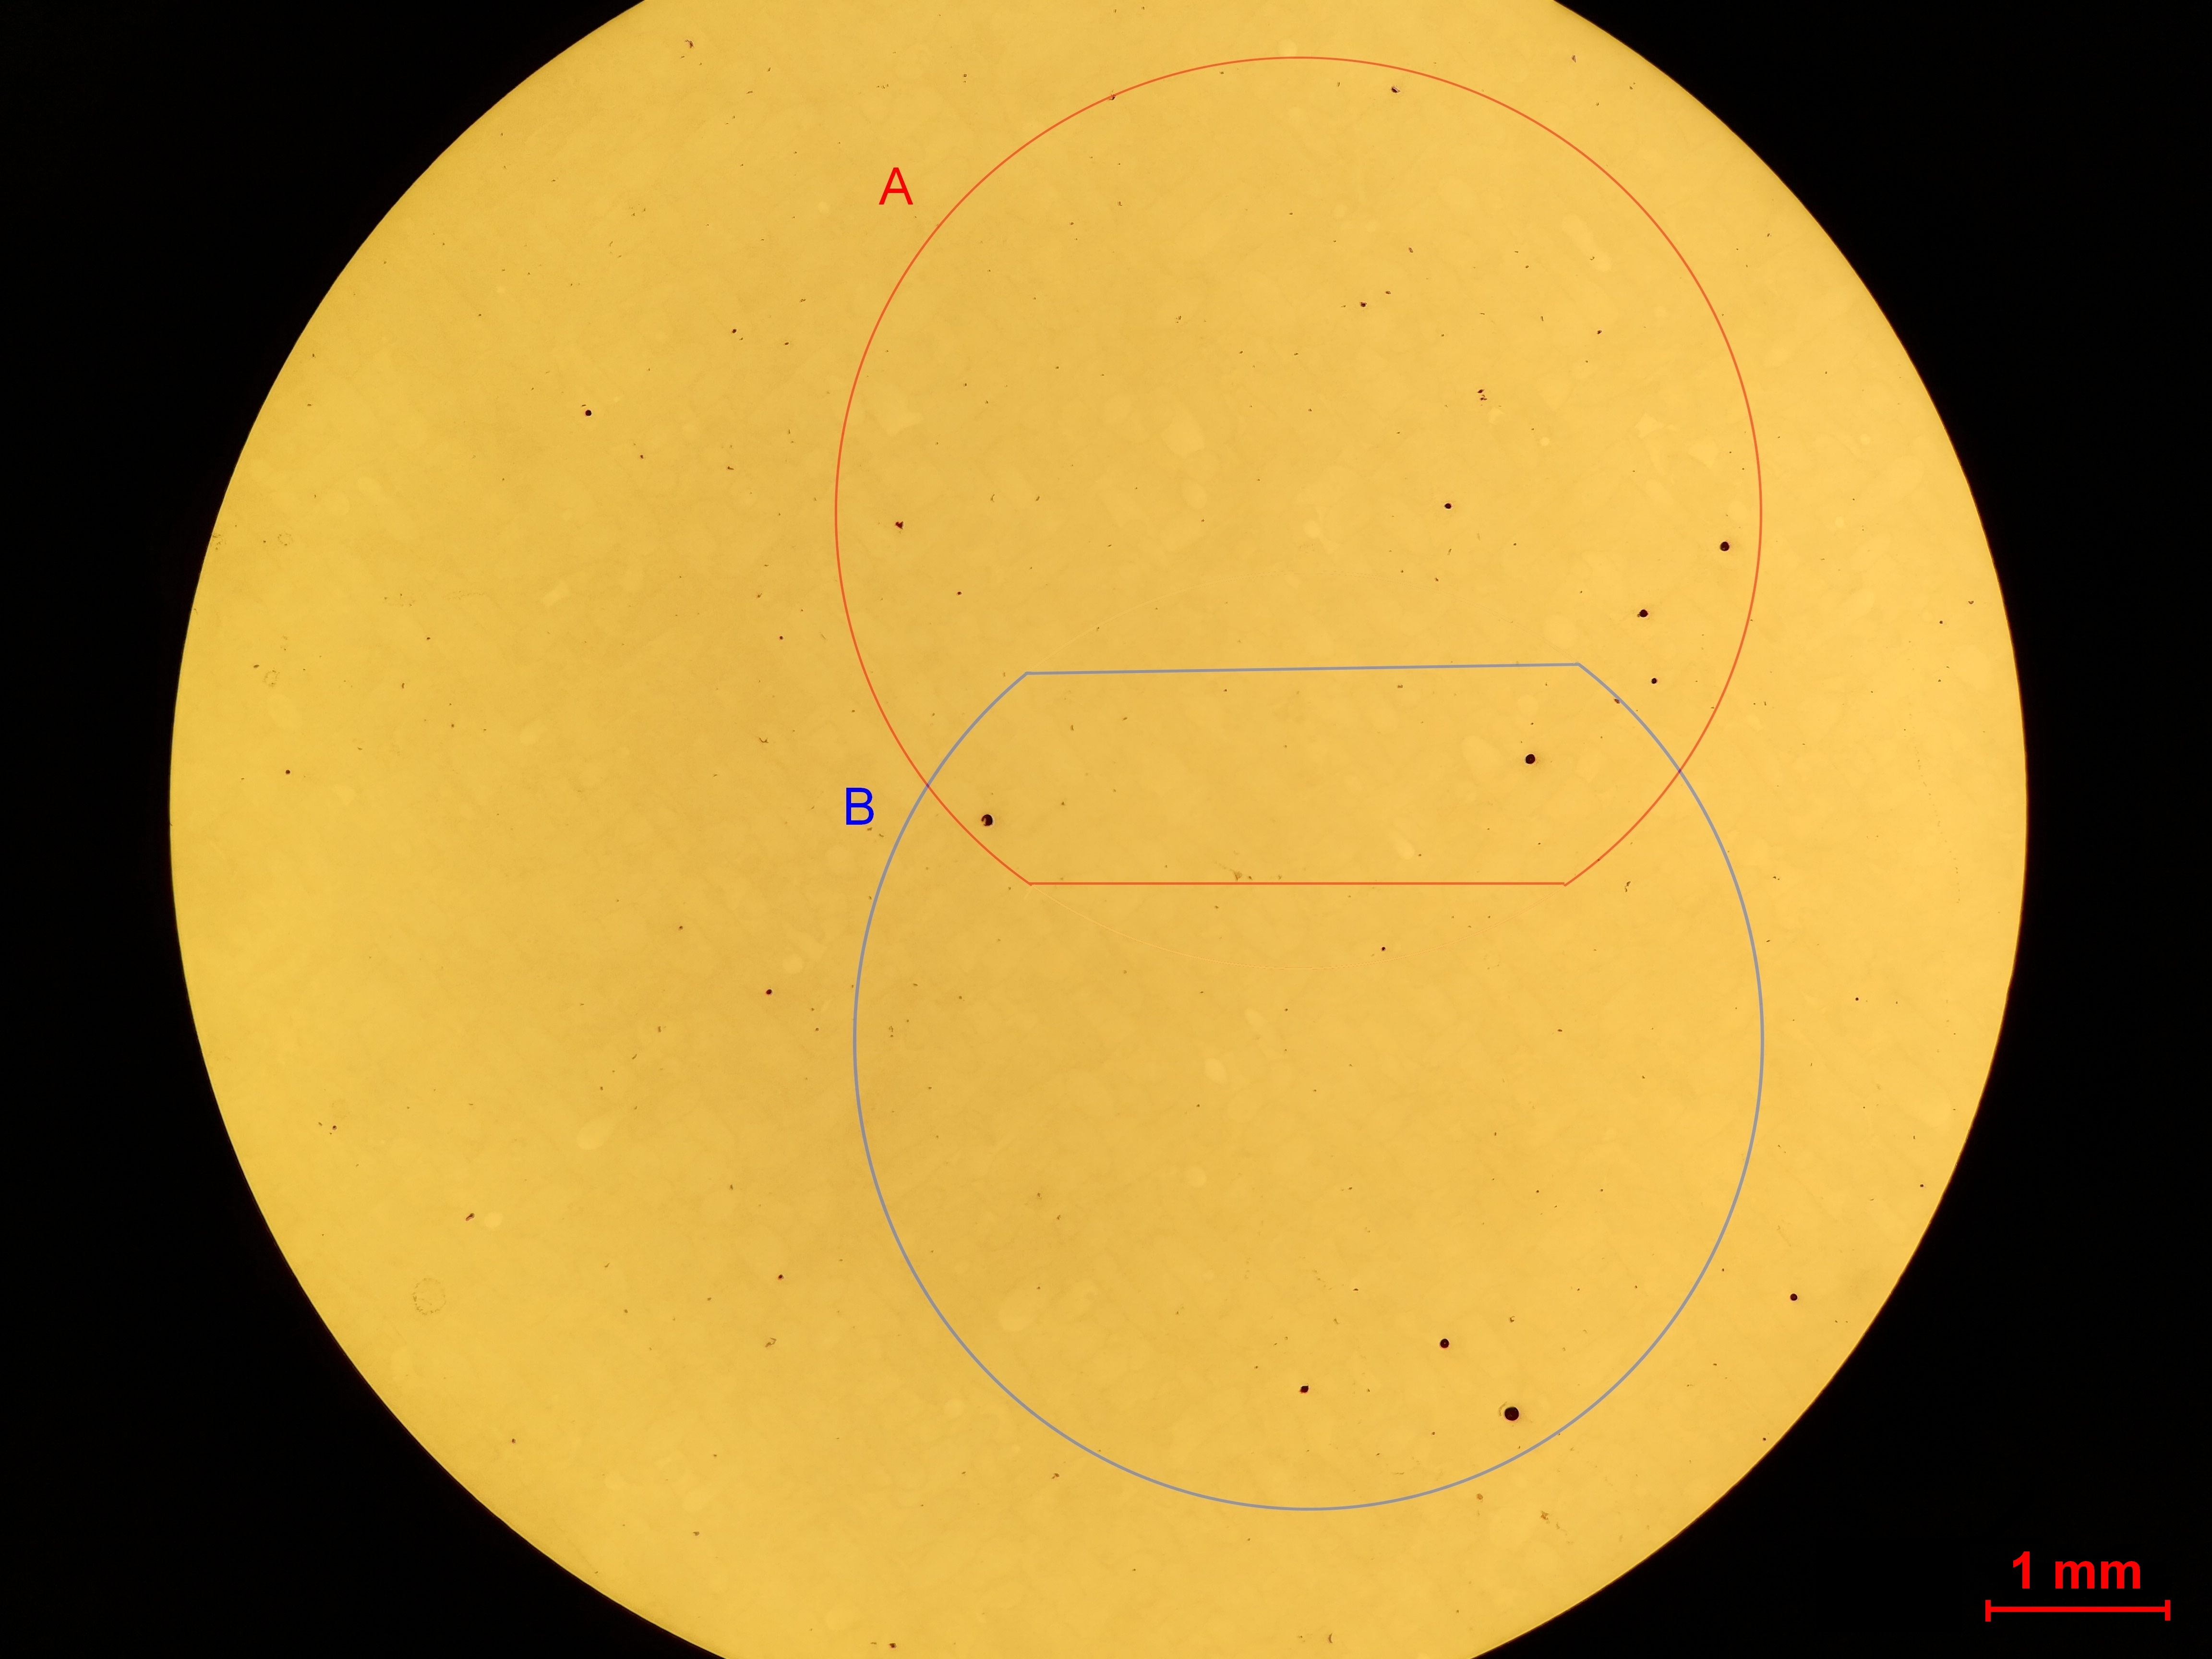
\includegraphics[scale=0.075]{Images/RODIA1}}
	\decoRule
	\caption[5x magnification picture of specimen X200-180319-cub1 and delimitation of the zones A and B]{5x magnification picture of specimen X200-180319-cub1 and delimitation of the zones A and B}
	\label{fig:RODIA1}
\end{figure}

\begin{figure}[ht]
	\centering
	\centerline{\includegraphics[scale=0.43]{Images/RODIAHist}}
	\decoRule
	\caption[Histograms of porosities areas occurrences from pictures of specimen X200-180319 on zone A under (a) 5x magnification (b) 10x magnification]{Histograms of porosities areas occurrences from pictures of specimen X200-180319 on zone A under (a) 5x magnification (b) 10x magnification. }
	\label{fig:RODIAH}
\end{figure}


The comparison of figures \ref{fig:RODIA2} (b) and (d) shows that much more small porosities are isolated if the resolution is refined. This is confirmed by the histograms on figure \ref{fig:RODIAH}. The threshold of porosity area for detection in the case of 5x magnification is 0.5625 [$\mu m^2$] whereas it is 0.14 [$\mu m^2$] for 10x magnification. This area corresponds to a pixel in each case. It is also worth noting that there is an overall tendency to overestimate the areas at lower resolution, which counterbalances slightly the low number of detected porosities. \\

\begin{figure}[ht]
	\centering
	\centerline{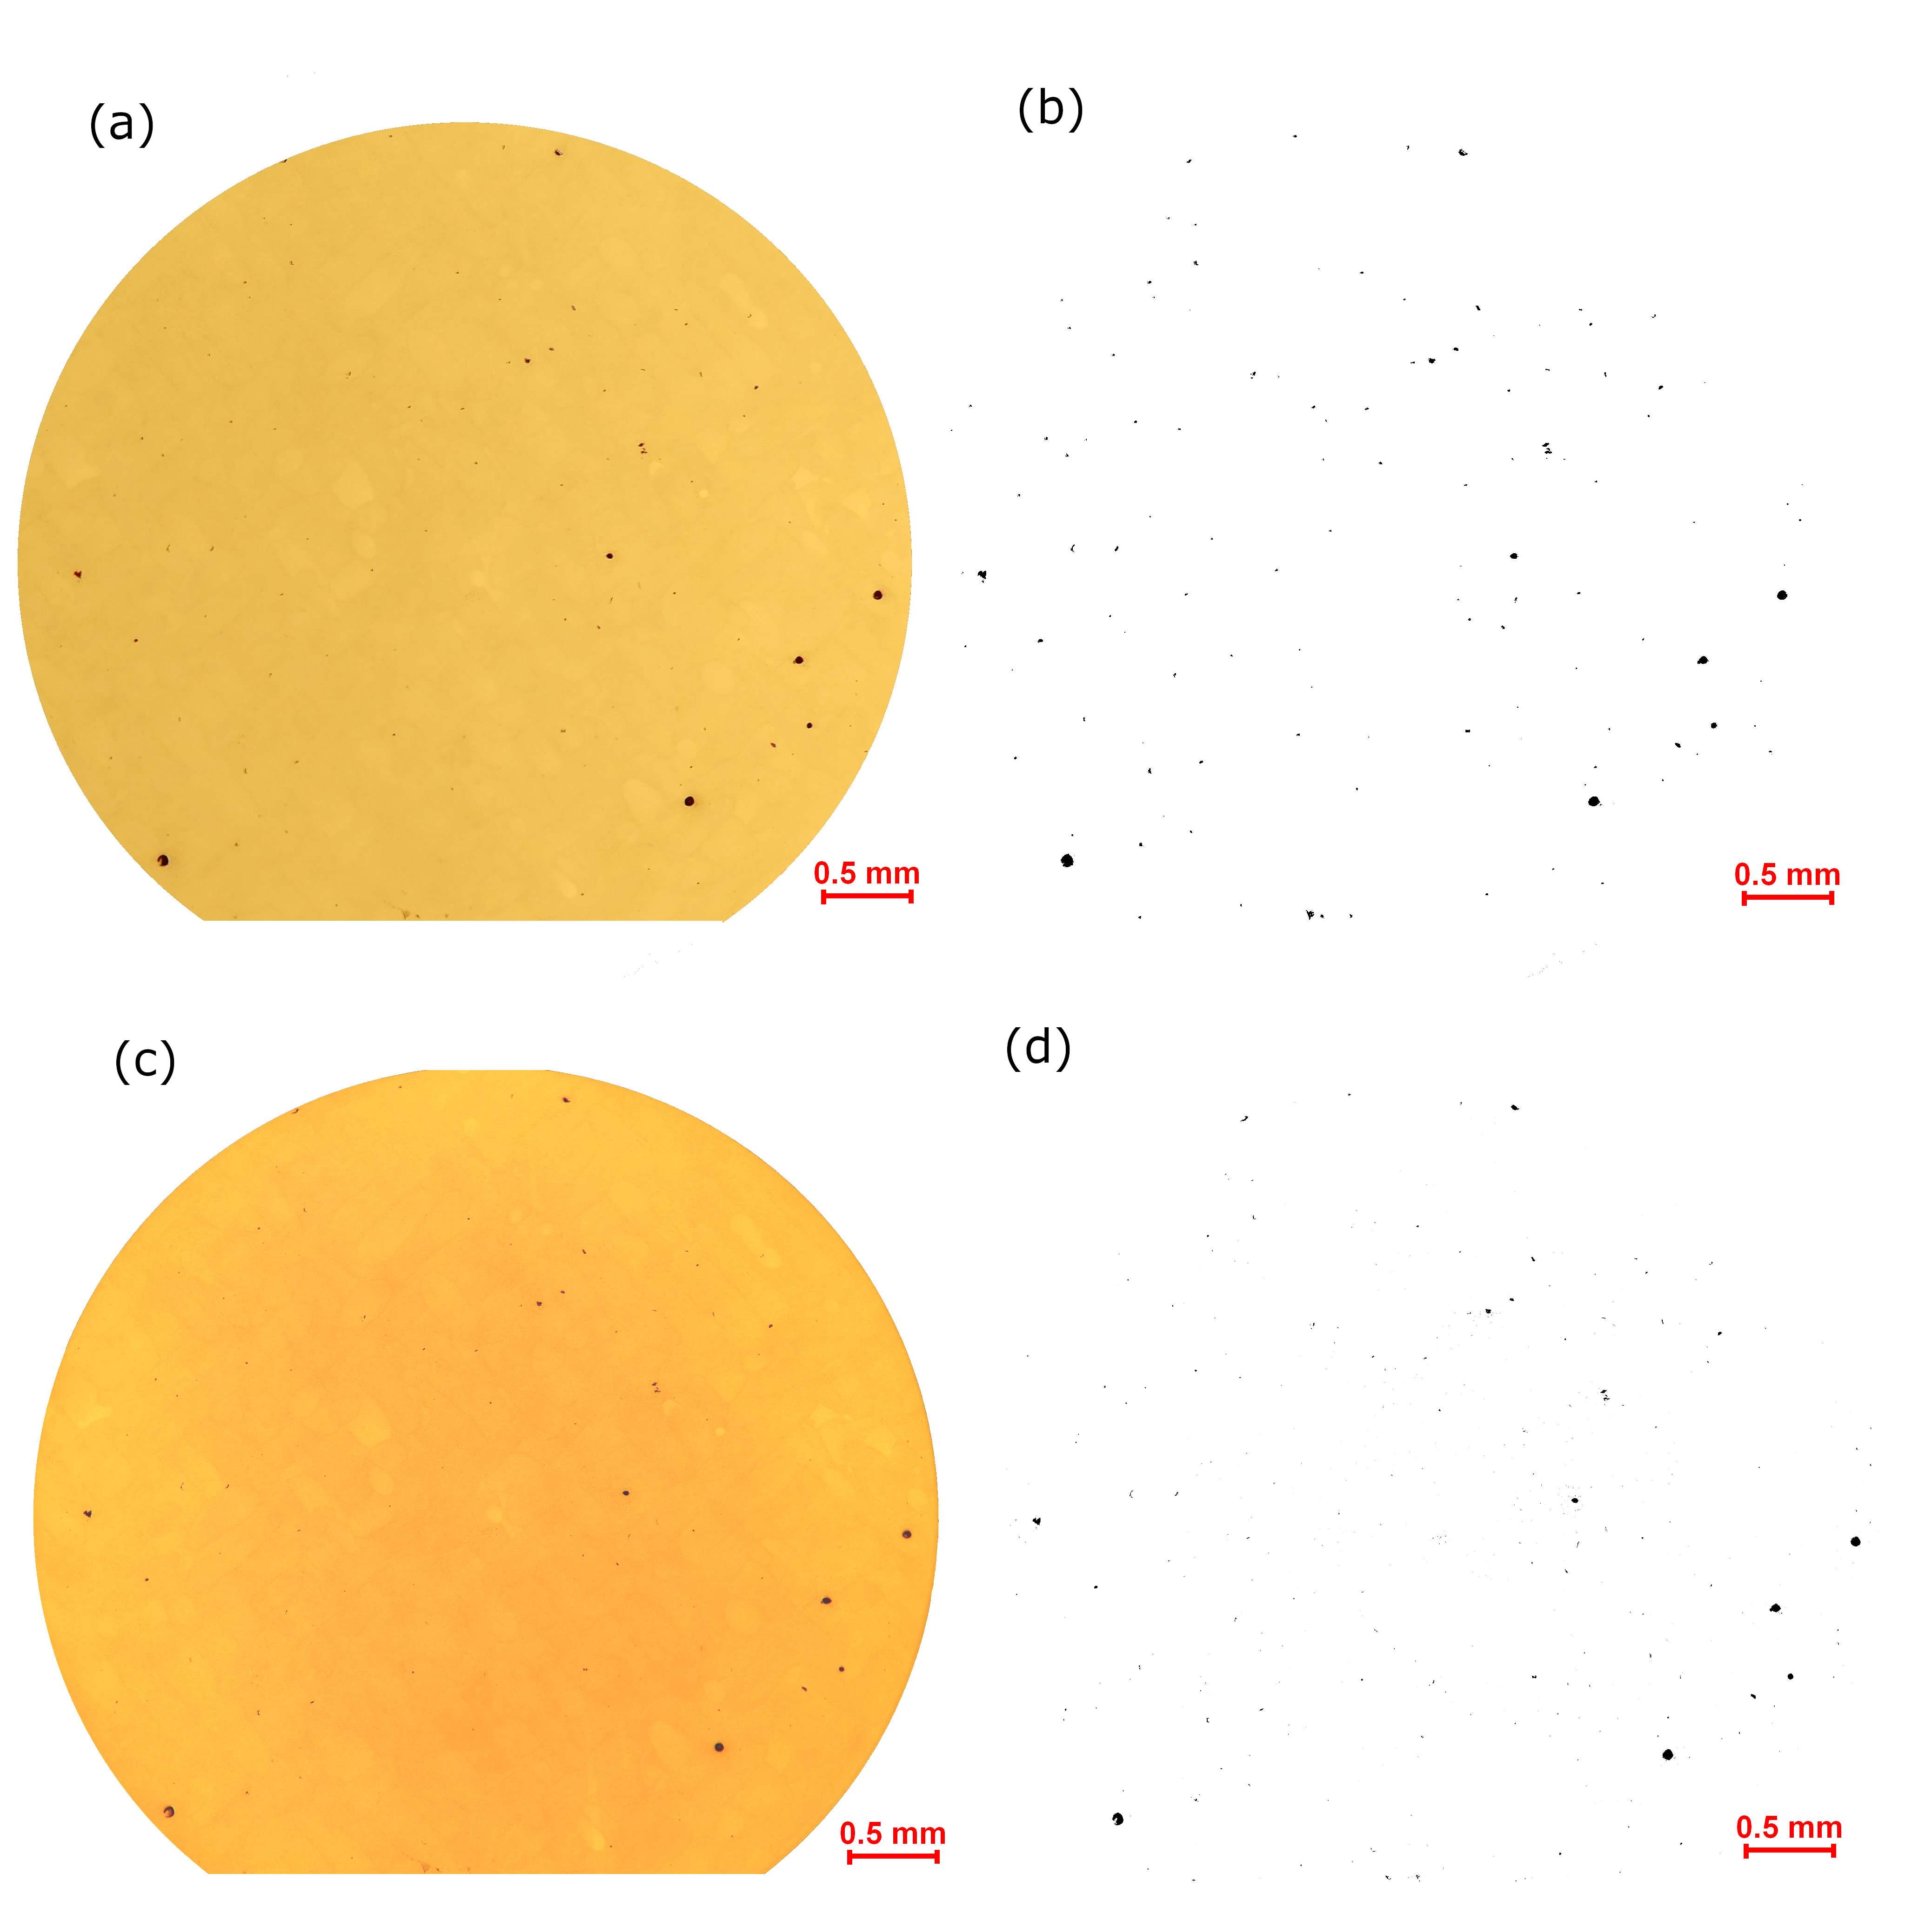
\includegraphics[scale=0.44]{Images/RODIA2}}
	\decoRule
	\caption[Zone A of specimen X200-180319-cub1: (a) Delimitation from original picture under 5x magnification (b) Porosities isolation from 5x magnification picture (c) Original picture under 10x magnification (d) Porosities isolation of 10x magnification picture]{Zone A of specimen X200-180319-cub1: (a) Delimitation from original picture under 5x magnification (b) Porosities isolation from 5x magnification picture (c) Original picture under 10x magnification (d) Porosities isolation of 10x magnification picture}
	\label{fig:RODIA2}
\end{figure}


The RODIA results for zones A and B are outlined in table \ref{tab:RODIASS}. It was observed that pictures with lower resolution have the tendency to lead to the overestimation of the relative density. The order of magnitude of the difference is of few hundredths of percent. The method is thus presumably positively biased. However, the observed effect is minor: this is probably due to the fact that the undetected porosities are the smallest, which influence the less the calculated density value.\\

\begin{center}
	\begin{table}[ht]
		\centerline{\begin{tabular}{|c|c|c|}
				\hline
				Zone & Magnification & Measured relative density [$\%$] \\
				\hline
				A & 5x  & 99.87\\
				A & 10x & 99.84\\
				B & 5x & 99.86\\
				B & 10x & 99.85\\
				\hline
		\end{tabular}}
		\caption[RODIA results for zones A and B of specimen X200-180317 with 5x and 10x magnification]{RODIA results for zones A and B of specimen X200-180317 with 5x and 10x magnification}
		\label{tab:RODIASS}
	\end{table}
\end{center}

Taking pictures at refined magnification could be considered to better the precision of the method. This would, however, require to augment the number of analysed pictures to have a sample of pictures as representative. A picture with doubled magnification covers indeed four times less surface. The number of analyses should thus be quadrupled to take as much information into account.\\

RODIA method required to make the assumption that the volumetric porosity fraction is equal the surface one. The dependability of this affirmation will now be discussed. Let us consider a cubic cell of side length D containing a spheric porosity of diameter D in its center (see figure \ref{fig:DDD}). The volumetric porosity fraction $f_v$ is:\\

$$f_v = \frac{\frac{\pi D^3}{6}}{D^3}= \frac{\pi}{6}$$

\begin{figure}[ht]
	\centering
	\centerline{\includegraphics[scale=0.64]{Images/DDD}}
	\decoRule
	\caption[Schematic of a spheric porosity of diameter D in a cubic cell of size length D]{Schematic of a spheric porosity of diameter D in a cubic cell of size length D}
	\label{fig:DDD}
\end{figure}

However, the surface porosity fraction depends on the observed pore diameter $D_{obs}$ which varies with the z coordinate of the surface plane crossing it: $\frac{D_{obs}(z)}{2}=\sqrt{(\frac{D}{2})^2-z^2}$. If we assume that there is a statistically significant number of pores of similar size, one can make the hypothesis that - in average - the observed diameter is the mean diameter $D_{mean}$:\\

$$ \frac{D_{mean}}{2}= \frac{\int_{-\frac{D}{2}}^\frac{D}{2} D_{obs}(z) dz}{D}=\frac{\pi D}{8}$$

This hypothesis is quiet coherent for small pores but not  for the largest: in most cases, a very small number of pores is significantly bigger than the others. If we still assume it to be true, the surface porosity fraction $f_s$ can be computed as follows:

$$f_s=\frac{\frac{\pi D_{mean}^2}{4}}{D^2}=\frac{\pi^3}{16 \cdot 4} \simeq 0.9253 f_v$$

It can thus be concluded that the method to measure the relative density is slightly intrinsically positively biased. The greater the porosity is, the bigger the bias. In the working range of $\rho_{rel}$ of this work, they can go from 0.01 to 0.03 [\%]. Combining this with the bias induced by the measures imperfections, one can conclude that RODIA should be used as a mean to estimate an upper limit for the relative densities.

\subsection{Measures comparison}
Some samples' densities were also measured through hydrostatic weighing (both with and without preliminary polishing). Multiple techniques were performed on the same few specimens in order to draw a comparison of the results and reach a deeper understanding of the methods reliability. The results are gathered on figures \ref{fig:7comp} and \ref{fig:2comp}.\\

\begin{figure}[ht]
	\centering
	\centerline{\includegraphics[scale=0.64]{Images/7comp}}
	\decoRule
	\caption[Bar chart of the density measurements with the HW (AB and after polishing) and RODIA methods for samples of batch X200-180109]{Bar charts of the density measurements with the HW (AB and after polishing) and RODIA methods for samples of batch X200-180109}
	\label{fig:7comp}
\end{figure}

\begin{figure}[ht]
	\centering
	\centerline{\includegraphics[scale=0.64]{Images/2comp}}
	\decoRule
	\caption[Bar charts of the density measurements with the HW (after polishing) and RODIA methods for samples of (a) batch X200-180319 (b) batch X200-180417]{Bar charts of the density measurements with the HW (after polishing) and RODIA methods for samples of (a) batch X200-180319 (b) batch X200-180417}
	\label{fig:2comp}
\end{figure}

As-built hydro measurements on figure \ref{fig:7comp} demonstrated high variability relatively to the other measures. Over the five tested samples, two exhibited similar relative densities for all techniques. However, three had $\rho_{a,rel}$ significantly below the values obtained with the other methods. In particular, the gap for sample "7c" was 0.44 [\%]. The fact that the CI do not intersect with the others' suggest that AB HW method was negatively biased in those cases. The most plausible explanation is that air was trapped in the surface roughness, which distorted the results (by overestimating the closed porosities volume. This would not be surprising as SLM produced parts usually have bad surface finish.\\ %to observe potential inhomogeneous distributions of the closed porosities in the specimens.

The two other methods were more promising. Relative densities obtained with RODIA method are generally close to the ones of HW after polishing (see figures \ref{fig:7comp} and \ref{fig:2comp}). In average, the absolute difference between the two is 0.16 [\%] (0.24 [\%] at most).  When the difference is greater than 0.02 [\%], the RODIA method always give greater density values. In addition, the CI do not always intersect. This can be attributed to the RODIA positive bias, and potentially to a negative bias for HW - that would still not be fully erased through polishing. Ultimately, given the opposite bias and the proximity of the relative density values for both methods, one could consider the two to be bounds between which lies the actual $\rho_{rel}$.\\

\section{Density and hardness study}

\subsection{Parameters optimisation}
Optimisations of the relative density and hardness were both achieved with the parameters set ($P=0.75 P_{max}=205 [W]$ , $v_s=1200 [\frac{mm}{s}]$). This pair of parameters lie in the process window suggested in section \ref{pp}.
Kempen et al. found optimal parameters values (maximising density) that are not far to the ones of this work (see table \ref{tab:compKemp}) \parencite{Kempen110817}. The energy density was however significantly bigger in this work, especially since the laser was more focused (which is not taken into account for the approximate computation). $E_d$ is rather close to a value minimising porosity obtained by Read et al. (65 $\frac{J}{mm^3}$) \parencite{Read150417}. Both cited sources used a chessboard scanning strategy, with islands size of around  5x5 [$mm^2$]. \\

\begin{center}
	\begin{table}[ht]
		\centerline{\begin{tabular}{|c|c|c|c|c|c|c|}
				\hline
				Source & h [$\mu m$] & t [$\mu m$]  & $\phi_{99\%} [\mu m]$& P $[W]$ &$v_s [\frac{mm}{sec}]$ & $E_d [\frac{J}{mm^3}]$ \\
				\hline
				This work & 100  & 30 & 75 & 205 & 1200 & 57\\
				\parencite{Kempen110817} & 105 & 30 & 150 & 200 & 1400  & 45 \\
				\parencite{Read150417} & 75 & 30  & 150 & 200 & 1350 & 65 \\				
				\hline
		\end{tabular}}
		\caption[Optimised manufacturing parameters comparison with literature sources]{Optimised manufacturing parameters comparison with literature sources}
		\label{tab:compKemp}
	\end{table}
\end{center}

A relative density of 99.9 [\%] was reached, which is superior to the best values found in the literature \parencite{EOS}. It is likely that all samples fabricated with the optimised parameters had $\rho_{rel}>99.4[\%]$ according to the measurements. Results depended on the powder age and recycling (\ref{RPI}). It can be confirmed that the parameters chosen allowed for a right energy input and a correct melt pools overlapping. The hardness was significantly bigger than what is typically expected - approximately 10 [HV] more (see section \ref{MMABMP}). \textcolor{gray}{[EXPLICATIONS?= THERMIQUE? OU CONTRAINTES RESIDUELLES? Normalement pas car quasi nulles près de la surface normalement -> calculer profondeur de pénétration d'après pointe Vickers]}\\

However, one should note that the optimisation of the overall density was perhaps not the most pertinent to conduct. \textcolor{gray}{[TAILLE MAX DES PORES, CONTRAINTES RESIDUELLES -> Sur des éprouvettes... VOIR SECTION FUTURE]}.\\ 

\subsection{Reproducibility}

[Connu que quand T augmente, la porosité augmente (vient de la solubilité en H?) -> Existence d'un seuil? Ca expliquerait l'effet pour les échantillons de type 8 et pas pour les 7]
[Variabilité des éch type 8 = instabilité key holes]
[Impact de la poudre: peut-être qu'à la fin elle était humide, impossible à voir via ICP]

\section{Characterisation of the as-built samples}

\subsection{Mechanical properties}

The average tensile properties measures for AB specimens fell a bit short of the expectations. While $\sigma_y$ and $\sigma_u$ were more or less satisfactory compared to what is observed in literature, $\epsilon_f$ was lower than what is typically obtained. Furthermore, while $E$ varies a lot in literature, it is extremely rare that it reaches an average value as low as 65. \\

Results were compared to the \textit{Aerostream} project's carried out by ULB, VUB and UCL universities in which AlSi10Mg tensile specimens were also fabricated vertically and tested. The process parameters used for the project are unfortunately undisclosed. The comparison of the AB specimens is presented on figure \ref{AerAB}. The properties obtained with the \textit{Aerostream} project are obviously far better than what was obtained in this thesis for as-built specimens (and to what can be found in literature). The fracture strain was indeed three times bigger and the ultimate tensile strength 124\% higher. Insight on the reasons behind the differences will be provided in section \ref{D-MP}.

\begin{figure}[ht]
	\centering
	\centerline{\includegraphics[scale=0.64]{Images/AerAB}}
	\decoRule
	\caption[Engineering stress-strain tensile curves for as-built specimens of this work (in average) and of \textit{Aerostream} project]{Engineering stress-strain tensile curves for as-built specimens of this work (in average) and of \textit{Aerostream} project}
	\label{fig:AerAB}
\end{figure}

\subsection{Microstructure}

[Mécanisme d'endommagement: deux populations de porosités? A confirmer/ infirmer avec les articles envoyés par AS]
[Taille des cupules= ordre de grandeur des éléments de la microstructure?] 

\section{Characterisation of the heat treated samples}

\subsection{Heating process}
Quand on chauffe à 300 deg, on chauffe déjà longtemps à plus de 200 deg

\subsection{Residual stresses}

[XRD: pièce as-built a un plus petit spread que ceux avec TT à basse T, p-e parce que cube coupé en 2 => relaxation des contraintes après fab?]

While the usual stress-relief treatment for aluminium alloys -to hours holding at 300$^\circ$ C- does indeed relieve stresses inside the specimen, it also triggers significantly the diffusion of alloying elements, altering the material microstructure.

\subsection{Mechanical properties}
[Propriétés as-built moins bonnes que dans la litérature car contraintes résiduelles. On a pas les conditions de fabrication des meilleurs -> Ils avaient surement un controle de la température de la plaque] 
[Faire le dessin de courbe "montée" par les contraintes]
[Augmentation de ductilité = disparition des	limites entres bains de fusion? ou compensation du matériau ductile autours des trous? A confirmer/infirmer via les images du SEM de la section d'après]
[Différence de porosité avant/ après TT qui explique quelque chose? -> Analyse image J des résultats]
[Lien avec la dureté -> Résultats]

\subsection{Microstructure}
[Modèle pour la sphéroisisation: rien dans la literature pour notre microstructure (? j'ai rien trouvé en faisant une petite recherche)]
[Trajet de fissure "accidenté"? Déviation par les défauts?]


\label{D-MP}

\subsection{Optimisation}



%\section{Mechanical testing}